\vspace*{4mm}
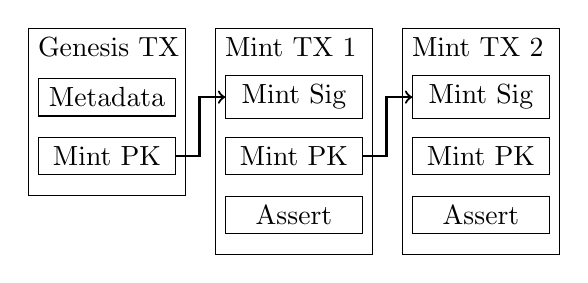
\begin{tikzpicture}
% \node at (-1, 2.5) {Inputs};
% \node at (5, 2.5) {Outputs};
\draw (0, 0.75) rectangle (2,2.875);
\node[below right] at (0, 2.875) {Genesis TX};
\node[draw, text width=1.5cm, align=center] (Metadata 1) at (1,2) {Metadata};
\node[draw, text width=1.5cm, align=center] (Mint PK 1) at (1,1.25) {Mint PK};

\draw (2.375, 0) rectangle (4.375,2.875);
\node[below right] at (2.375, 2.875) {Mint TX 1};
\node[draw, text width=1.5cm, align=center] (Mint Sig 1) at (3.375,2) {Mint Sig};
\node[draw, text width=1.5cm, align=center] (Mint PK 2) at (3.375,1.25) {Mint PK};
\node[draw, text width=1.5cm, align=center] (Assert 1) at (3.375,0.5) {Assert};

\draw (4.75, 0) rectangle (6.75,2.875);
\node[below right] at (4.75, 2.875) {Mint TX 2};
\node[draw, text width=1.5cm, align=center] (Mint Sig 2) at (5.75,2) {Mint Sig};
\node[draw, text width=1.5cm, align=center] (Mint PK 3) at (5.75,1.25) {Mint PK};
\node[draw, text width=1.5cm, align=center] (Assert 2) at (5.75,0.5) {Assert};

\draw[->, thick] (Mint PK 1) -| (2.175, 2) |- (Mint Sig 1);
\draw[->, thick] (Mint PK 2) -| (4.55, 2) |- (Mint Sig 2);
\end{tikzpicture}
\vspace*{4mm}
